\documentclass{beamer}

\usepackage[utf8]{inputenc}
\usepackage{textcomp}
\usepackage[official]{eurosym}
\usepackage[polish]{babel}
\usepackage{amsthm}
\usepackage{graphicx}
\usepackage[T1]{fontenc}
\usepackage{scrextend}
\usepackage{hyperref}
\usepackage{xcolor}
\usepackage{listings}
\graphicspath{ {./fig/} }

\usetheme{default}
\usecolortheme{seahorse}

\beamertemplatenavigationsymbolsempty

\title{Viua VM w akcji}
%%\subtitle{Implementacja wysokopoziomowego języka programowania i realizacja prostej aplikacji}
\subtitle{Implementacja wysokopoziomowego języka programowania i realizacja prostej aplikacji
\\
\emph{Viua VM in action. Implementation of a high-level programming language and a simple application}}
\author{Marek Marecki \and Krzysztof Franek \\ Promotor: dr hab. Marek Bednarczyk prof. PJATK}

\begin{document}
\lstset{basicstyle=\ttfamily\color{black},
columns=fixed,
escapeinside={\%*}{*)},
inputencoding=utf8,
extendedchars=true,
moredelim=**[is][\color{red}]{@}{@}}

\frame{\titlepage}

\begin{frame}
    \frametitle{Viua VM -- tytułem wstępu}

    Viua VM to projekt rozpoczęty w połowie grudnia 2014.

    ~\\

    Jest to maszyna wirtualna wykorzystująca model aktorów jako główny model przetwarzania.
    Możliwe jest jej programowanie w języku assemblera, a programy są sekwencjami instrukcji modyfikujących
    stan zestawu rejestrów oferowanego przez ISA maszyny.

    ~\\

    Projekt jest udostępniany na licencji GNU GPL v3.
\end{frame}

\begin{frame}
    \frametitle{Omówienie problemu}
    % \framesubtitle{Problemy i więcej problemów}

    Współczesny hardware zmierza coraz bardziej w stronę współbieżności i
    wykonywania równoległego. Jednocześnie, mainstreamowe języki z uwagi na swój
    wiek wykorzystują \textbf{stare narzędzia} do obsługi równoległości, lub
    \textbf{nie uwzględniają jej \emph{w ogóle}}.

    ~\\

    Pisanie niezawodnych, mało awaryjnych programów jest trudne. Częściowo jest
    to spowodowane \textbf{zbyt słabą izolacją} podsystemów wewnątrz oprogramowania.

    ~\\

    Pytanie: ,,Czy Viua VM umożliwia pisanie niezawodnego, wysoce współbieżnego,
    nietrywialnego oprogramowania?''
\end{frame}

\begin{frame}
    \frametitle{Cel i zakres pracy inżynierskiej}
    \framesubtitle{Wynikające z problemu}

    Projekt obejmuje:
    \begin{enumerate}
        \item implementację wysokopoziomowego języka programowania
        \item realizację prostej aplikacji
    \end{enumerate}
\end{frame}

\begin{frame}
    \frametitle{Główne zadania}
    \framesubtitle{Z podziałem na członków zespołu}

    Marek Marecki:
    \begin{enumerate}
        \item specyfikacja języka programowania ViuAct
        \item projekt i implementacja kompilatora języka ViuAct
    \end{enumerate}

    ~\\

    Krzysztof Franek:
    \begin{enumerate}
        \item testowanie kompilatora języka ViuAct ,,w praktyce''
        \item projekt i implementacja programu ViuaChat w języku ViuAct
    \end{enumerate}
\end{frame}

\begin{frame}
    \frametitle{Strategia realizacji i technologia}
    % \framesubtitle{Podział zadań}

    Specyfikacja języka programowania ViuAct:
    \begin{enumerate}
        \item strategia: kaskada i iteracja
    \end{enumerate}

    ~\\

    Kompilator języka programowania ViuAct:
    \begin{enumerate}
        \item języka implementacji kompilatora: Python
        \item strategia: \emph{cowboy coding}\footnote{\url{ttps://wiki.c2.com/?CowboyCoding}}
    \end{enumerate}

    ~\\

    Program ViuaChat:
    \begin{enumerate}
        \item język implementacji: ViuAct
        \item strategia: ,,miniSCRUM'' (kanban, bez \emph{daily stands}, bez
            ,,Scrum Mastera'', typowe artefakty: user stories, backlog, sprinty)
    \end{enumerate}
\end{frame}

\begin{frame}
    \frametitle{ViuAct}
    \framesubtitle{Krótko o języku}

    Język ViuAct zapewnia dostęp do większości mechanizmów oferowanych przez Viua VM.

    ~\\

    Jest językiem opartym na wyrażeniach (większość konstrukcji to wyrażenia), ze składnią podobną do Lispa.
    Programy pisane w ViuAct składają się z funkcji porozmieszczanych w modułach.

    ~\\

    Model wykonywania programów jest wzorowany na modelu aktorów.
\end{frame}

\begin{frame}
    \frametitle{ViuAct}
    \framesubtitle{Struktura kompilatora}

    \begin{figure}[!htp]
        \centering
        % 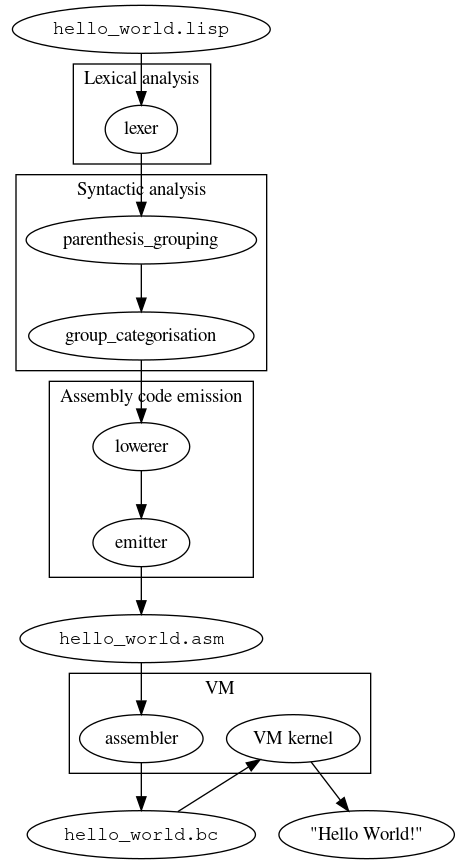
\includegraphics[width=9cm]{viuact-pipeline}
        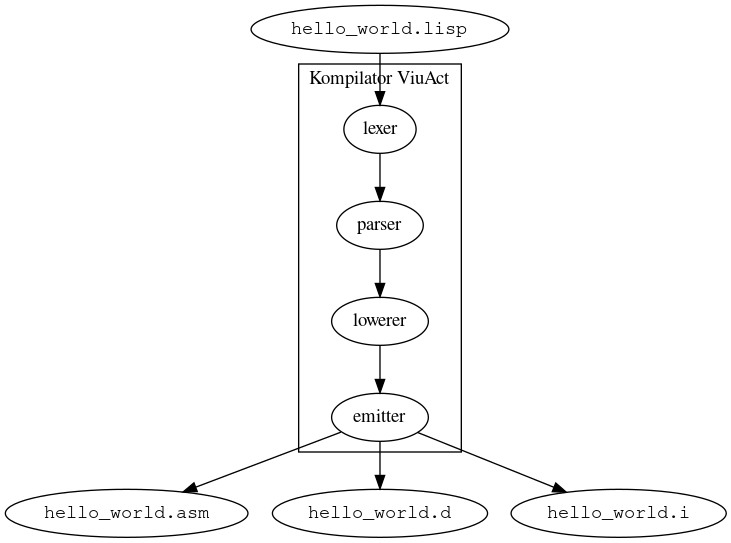
\includegraphics[width=10cm]{viuact-ogolny-schemat-kompilatora}
    \end{figure}
\end{frame}

\begin{frame}
    \frametitle{ViuaChat}
    \framesubtitle{Chat w ViuAct}

    \begin{enumerate}
        \item Prosta aplikacja czatu webowego
        \item Zbudowana w dwóch celach:
        \begin{enumerate}
        	\item Zademonstrowanie możliwości kompilatora
        	\item Przykładowy kod dla przyszłych programistów
        \end{enumerate}
    \end{enumerate}
\end{frame}

\begin{frame}
    \frametitle{ViuaChat}
    \framesubtitle{Podstawowa architektura}

    \begin{enumerate}
        \item Frontend: Single Page App
        \begin{enumerate}
        	\item Vue.js
        	\item HTML5
        \end{enumerate}
        \item Backend
        \begin{enumerate}
        	\item Serwer Nginx - wystawia statyczny HTML i JS
        	\item Maszyna ViuaVM - właściwy serwer czatu
        \end{enumerate}
        \item Komunikacja front-back: via Websocket
    \end{enumerate}
\end{frame}

\begin{frame}
    \frametitle{ViuaChat}
    \framesubtitle{Architektura}

    \begin{figure}[!htp]
        \centering
        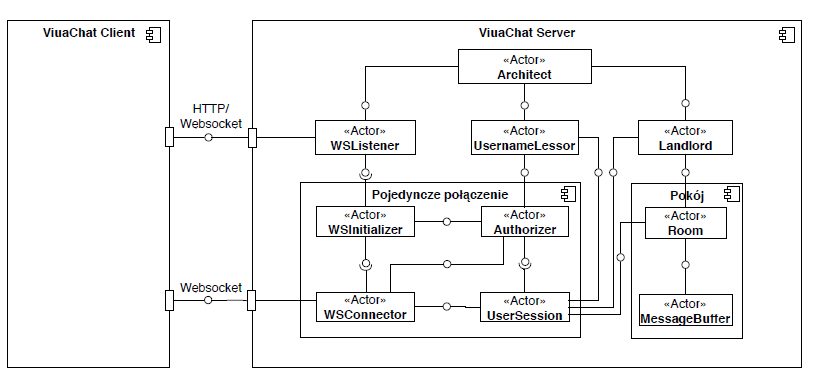
\includegraphics[width=\textwidth]{pckdiag}
    \end{figure}
\end{frame}

\begin{frame}
    \frametitle{Wyniki}
    \framesubtitle{Sukcesy}

    \begin{enumerate}
        \item wytworzenie specyfikacji
        \item wytworzenie kompilatora
        \item wytworzenie chatu
        \item projekt na NAI Krzysztofa napisany w języku ViuAct
    \end{enumerate}
\end{frame}

\begin{frame}
    \frametitle{Wyniki}
    \framesubtitle{Porażki}

    \begin{enumerate}
        \item \emph{\textbf{niezadowalająca}} szybkość kompilacji
        \item sposób raportowania błędów w kompilatorze
        \item nieoczywiste ograniczenia w łączeniu konstrukcji językowych
    \end{enumerate}
\end{frame}

\begin{frame}[fragile]
    \frametitle{Przykład kodu}
    \framesubtitle{Wszystkie konstrukcje w ViuAct}

    \begin{small}
    \begin{lstlisting}
(let countdown (n) {
    (let x (try (Std.Actor.receive 1s) (
        (catch Exception _
            (tailcall countdown n)))))

    (let wrapped (struct))
    (:= wrapped.value x)
    (:= wrapped.sequence (Std.copy n))
    (actor f wrapped)

    (if (= n 0) 0 (tailcall countdown (- n 1)))
})
    \end{lstlisting}
    \end{small}
\end{frame}

\begin{frame}[fragile]
    \frametitle{Przykład kodu}
    \framesubtitle{Nazwa i parametry formalne}

    \begin{small}
    \begin{lstlisting}
(let @countdown@ (@n@) {
    (let x (try (Std.Actor.receive 1s) (
        (catch Exception _
            (tailcall countdown n)))))

    (let wrapped (struct))
    (:= wrapped.value x)
    (:= wrapped.sequence (Std.copy n))
    (actor f wrapped)

    (if (= n 0) 0 (tailcall countdown (- n 1)))
})
    \end{lstlisting}
    \end{small}
\end{frame}

\begin{frame}[fragile]
    \frametitle{Przykład kodu}
    \framesubtitle{Ciało funkcji}

    \begin{small}
    \begin{lstlisting}
(let countdown (n) @{
    (let x (try (Std.Actor.receive 1s) (
        (catch Exception _
            (tailcall countdown n)))))

    (let wrapped (struct))
    (:= wrapped.value x)
    (:= wrapped.sequence (Std.copy n))
    (actor f wrapped)

    (if (= n 0) 0 (tailcall countdown (- n 1)))
}@)
    \end{lstlisting}
    \end{small}
\end{frame}

\begin{frame}[fragile]
    \frametitle{Przykład kodu}
    \framesubtitle{Odebranie wiadomości (wywołanie funkcji z modułu)}

    \begin{small}
    \begin{lstlisting}
(let countdown (n) {
    (let x (try (@Std.Actor.receive 1s@) (
        (catch Exception _
            (tailcall countdown n)))))

    (let wrapped (struct))
    (:= wrapped.value x)
    (:= wrapped.sequence (Std.copy n))
    (actor f wrapped)

    (if (= n 0) 0 (tailcall countdown (- n 1)))
})
    \end{lstlisting}
    \end{small}
\end{frame}

\begin{frame}[fragile]
    \frametitle{Przykład kodu}
    \framesubtitle{Obsługa wyjątków (słowa kluczowe)}

    \begin{small}
    \begin{lstlisting}
(let countdown (n) {
    (let x (@try@ (Std.Actor.receive 1s) (
        (@catch@ Exception _
            (tailcall countdown n)))))

    (let wrapped (struct))
    (:= wrapped.value x)
    (:= wrapped.sequence (Std.copy n))
    (actor f wrapped)

    (if (= n 0) 0 (tailcall countdown (- n 1)))
})
    \end{lstlisting}
    \end{small}
\end{frame}

\begin{frame}[fragile]
    \frametitle{Przykład kodu}
    \framesubtitle{Obsługa wyjątków (wyrażenie chronione)}

    \begin{small}
    \begin{lstlisting}
(let countdown (n) {
    (let x (try (@Std.Actor.receive 1s@) (
        (catch Exception _
            (tailcall countdown n)))))

    (let wrapped (struct))
    (:= wrapped.value x)
    (:= wrapped.sequence (Std.copy n))
    (actor f wrapped)

    (if (= n 0) 0 (tailcall countdown (- n 1)))
})
    \end{lstlisting}
    \end{small}
\end{frame}

\begin{frame}[fragile]
    \frametitle{Przykład kodu}
    \framesubtitle{Obsługa wyjątków (wyłapanie wyjątku)}

    \begin{small}
    \begin{lstlisting}
(let countdown (n) {
    (let x (try (Std.Actor.receive 1s) (
        @(catch Exception _@
            (tailcall countdown n)@)@)))

    (let wrapped (struct))
    (:= wrapped.value x)
    (:= wrapped.sequence (Std.copy n))
    (actor f wrapped)

    (if (= n 0) 0 (tailcall countdown (- n 1)))
})
    \end{lstlisting}
    \end{small}
\end{frame}

\begin{frame}[fragile]
    \frametitle{Przykład kodu}
    \framesubtitle{Obsługa wyjątków (wyrażenia obsługi)}

    \begin{small}
    \begin{lstlisting}
(let countdown (n) {
    (let x (try (Std.Actor.receive 1s) (
        (catch Exception _
            (@tailcall countdown n@)))))

    (let wrapped (struct))
    (:= wrapped.value x)
    (:= wrapped.sequence (Std.copy n))
    (actor f wrapped)

    (if (= n 0) 0 (tailcall countdown (- n 1)))
})
    \end{lstlisting}
    \end{small}
\end{frame}

\begin{frame}[fragile]
    \frametitle{Przykład kodu}
    \framesubtitle{\emph{let-binding} (dowiązanie zmiennej)}

    \begin{small}
    \begin{lstlisting}
(let countdown (n) {
    (let x (try (Std.Actor.receive 1s) (
        (catch Exception _
            (tailcall countdown n)))))

    (@let wrapped (struct)@)
    (:= wrapped.value x)
    (:= wrapped.sequence (Std.copy n))
    (actor f wrapped)

    (if (= n 0) 0 (tailcall countdown (- n 1)))
})
    \end{lstlisting}
    \end{small}
\end{frame}

\begin{frame}[fragile]
    \frametitle{Przykład kodu}
    \framesubtitle{Konstruktor \emph{\texttt{struct}}}

    \begin{small}
    \begin{lstlisting}
(let countdown (n) {
    (let x (try (Std.Actor.receive 1s) (
        (catch Exception _
            (tailcall countdown n)))))

    (let wrapped (@struct@))
    (:= wrapped.value x)
    (:= wrapped.sequence (Std.copy n))
    (actor f wrapped)

    (if (= n 0) 0 (tailcall countdown (- n 1)))
})
    \end{lstlisting}
    \end{small}
\end{frame}

\begin{frame}[fragile]
    \frametitle{Przykład kodu}
    \framesubtitle{Przypisanie do pola struktury}

    \begin{small}
    \begin{lstlisting}
(let countdown (n) {
    (let x (try (Std.Actor.receive 1s) (
        (catch Exception _
            (tailcall countdown n)))))

    (let wrapped (struct))
    (@:= wrapped.value x@)
    (:= wrapped.sequence (Std.copy n))
    (actor f wrapped)

    (if (= n 0) 0 (tailcall countdown (- n 1)))
})
    \end{lstlisting}
    \end{small}
\end{frame}

\begin{frame}[fragile]
    \frametitle{Przykład kodu}
    \framesubtitle{Wywołanie aktora}

    \begin{small}
    \begin{lstlisting}
(let countdown (n) {
    (let x (try (Std.Actor.receive 1s) (
        (catch Exception _
            (tailcall countdown n)))))

    (let wrapped (struct))
    (:= wrapped.value x)
    (:= wrapped.sequence (Std.copy n))
    (@actor@ f wrapped)

    (if (= n 0) 0 (tailcall countdown (- n 1)))
})
    \end{lstlisting}
    \end{small}
\end{frame}

\begin{frame}[fragile]
    \frametitle{Przykład kodu}
    \framesubtitle{Konstrukcja warunkowa}

    \begin{small}
    \begin{lstlisting}
(let countdown (n) {
    (let x (try (Std.Actor.receive 1s) (
        (catch Exception _
            (tailcall countdown n)))))

    (let wrapped (struct))
    (:= wrapped.value x)
    (:= wrapped.sequence (Std.copy n))
    (actor f wrapped)

    (@if (= n 0) 0 (tailcall countdown (- n 1))@)
})
    \end{lstlisting}
    \end{small}
\end{frame}

\begin{frame}[fragile]
    \frametitle{Przykład kodu}
    \framesubtitle{Konstrukcja warunkowa (wyrażenie sprawdzane; wywołanie operatora)}

    \begin{small}
    \begin{lstlisting}
(let countdown (n) {
    (let x (try (Std.Actor.receive 1s) (
        (catch Exception _
            (tailcall countdown n)))))

    (let wrapped (struct))
    (:= wrapped.value x)
    (:= wrapped.sequence (Std.copy n))
    (actor f wrapped)

    (if (@= n 0@) 0 (tailcall countdown (- n 1)))
})
    \end{lstlisting}
    \end{small}
\end{frame}

\begin{frame}[fragile]
    \frametitle{Przykład kodu}
    \framesubtitle{Konstrukcja warunkowa (...jeśli prawda)}

    \begin{small}
    \begin{lstlisting}
(let countdown (n) {
    (let x (try (Std.Actor.receive 1s) (
        (catch Exception _
            (tailcall countdown n)))))

    (let wrapped (struct))
    (:= wrapped.value x)
    (:= wrapped.sequence (Std.copy n))
    (actor f wrapped)

    (if (= n 0) @0@ (tailcall countdown (- n 1)))
})
    \end{lstlisting}
    \end{small}
\end{frame}

\begin{frame}[fragile]
    \frametitle{Przykład kodu}
    \framesubtitle{Konstrukcja warunkowa (...jeśli fałsz)}

    \begin{small}
    \begin{lstlisting}
(let countdown (n) {
    (let x (try (Std.Actor.receive 1s) (
        (catch Exception _
            (tailcall countdown n)))))

    (let wrapped (struct))
    (:= wrapped.value x)
    (:= wrapped.sequence (Std.copy n))
    (actor f wrapped)

    (if (= n 0) 0 (@tailcall countdown (- n 1)@))
})
    \end{lstlisting}
    \end{small}
\end{frame}

\begin{frame}[fragile]
    \frametitle{Przykład kodu}
    \framesubtitle{Wywołanie \emph{tailcall}}

    \begin{small}
    \begin{lstlisting}
(let countdown (n) {
    (let x (try (Std.Actor.receive 1s) (
        (catch Exception _
            (tailcall countdown n)))))

    (let wrapped (struct))
    (:= wrapped.value x)
    (:= wrapped.sequence (Std.copy n))
    (actor f wrapped)

    (if (= n 0) 0 (@tailcall@ countdown (- n 1)))
})
    \end{lstlisting}
    \end{small}
\end{frame}

% \begin{frame}
%     \frametitle{ViuaVM}
%     \framesubtitle{Harmonogram prac}

%     \begin{enumerate}
%         \item Do końca marca
%         \begin{enumerate}
%         	\item finalizacja kompilatora ViuAct i specyfikacji ViuaChat
%         	\item pierwsza wersja frontendu ViuaChat
%         \end{enumerate}         
%         \item Do końca kwietnia
%         \begin{enumerate}
%         	\item finalizacja pierwszej wersji backendu ViuaChat
%         	\item pierwsza integracja frontend-backend
%         	\item pierwsza wersja \textit{książki} do konsultacji z promotorem
%         \end{enumerate}
%         \item Do końca maja
%         \begin{enumerate}
%         	\item realizacja testów stabilności działania ViuaChat
%         	\item ukończenie prac nad stabilną wersją ViuaChat
%         	\item przygotowanie urządzeń testowych dla zaprezentowania projektu
%         	\item ukończenie \textit{książki}
%         \end{enumerate}
%     \end{enumerate}
% \end{frame}

\end{document}
